\documentclass[10pt]{article}
\usepackage{icmlko}

\icmlmeta{IP 파운데이션 월드모델}{192}{안쪽은 언제나 더 작은 모형을 고른다}{노트 191이 ``여러 번 잘라 평균하면 봉우리가 설 것''을 남겼다. 반대다 --- 뭉개진다. 그리고 뭉개지지 않는 것이 하나 있었는데, 그게 틀린 쪽으로 일관됐다}

\begin{document}

\twocolumn[
\icmlheader

\begin{abstract}
노트 191이 ``안쪽을 여러 시점에서 잘라 평균하면 봉우리 지수가 올라가고
챔피언도 조정할 수 있을 것''으로 닫았다. \textbf{반대다.} 능형의 봉우리가
분할마다 0.397 · 0.624 · 0.266 인데 \textbf{평균하면 0.365} 로 두 분할보다
낮다. 까닭이 있다 --- \textbf{분할마다 최적이 진짜로 다르다}(학습 크기가
다르므로). 평균은 잡음이 아니라 신호를 섞는다. \textbf{반복 분할을 채택하면
작동하던 능형 조정이 막힌다.} 그러면 무엇이 뭉개지지 않나. \textbf{선택
자체다} --- 능형은 세 분할 중 둘이, 트리는 \textbf{셋이 모두} 같은 것을
고른다. 그래서 ``선택 일치도''를 지표 후보로 재 봤다. \textbf{더 나쁘다}
--- 유보 이득과 스피어만 \textbf{$-$0.447} 로 방향이 반대다. F18 이 100\%
일치하면서 $-$0.010 을 잃고 F6 · F11 이 67\%로 $+$0.011 · $+$0.013 을 얻는다.
\textbf{일관되게 고른다고 옳게 고르는 것이 아니다.} 그런데 그 일관성이
단서였다. 트리가 세 분할에서 고르는 것이 \textbf{격자의 모서리}다 --- 깊이는
최대, 반복은 최소, 학습률은 최소. \textbf{안쪽 최적이 격자 밖에 있다는
뜻}이고, 용량으로 보면 $120{\times}0.03{=}3.6$ 대 기본값
$220{\times}0.06{=}13.2$ 로 \textbf{3.7배 작다.} 안쪽 학습행이 7,154 이고
전체가 10,292 이니 \textbf{행이 1.44배 적은데 용량은 3.7배 작게 고른다.}
그래서 되돌려 봤다. \textbf{용량을 행 비율의 \emph{제곱}(2.07)만큼 키우면
기본값을 넘는다} --- 반복과 학습률을 각각 $r$ 배 하면 $+$0.4563, 반복만
$r^2$ 배 하면 $+$0.4550, 기본값이 $+$0.4490 이다. \textbf{채택은 안 한다} ---
지수를 유보를 보고 골랐다. 확정된 것은 하나다: \textbf{안쪽 선택은 체계적으로
용량을 작게 잡는다.} 잡음이 아니라 편향이라 평균으로 못 고치고 일치도로 못
잡는다.
\end{abstract}
]

\begin{figure*}[t]
\centering
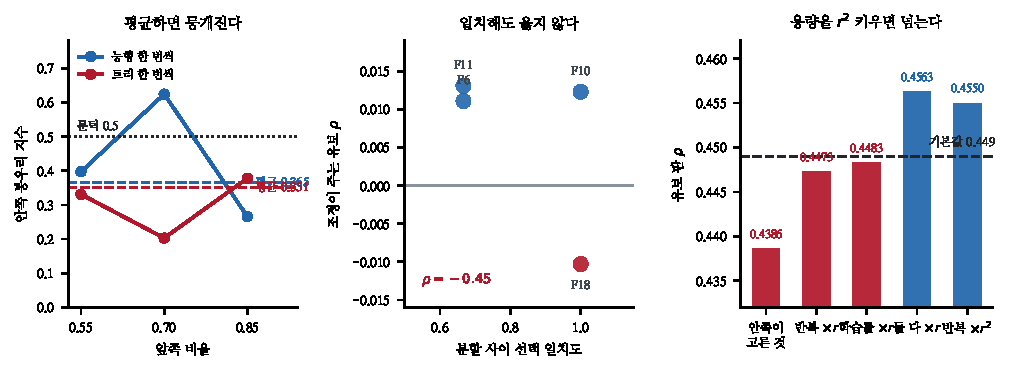
\includegraphics[width=\textwidth]{figs/small.pdf}
\caption{왼쪽 --- 평균하면 뭉개진다. 가운데 --- 일치해도 옳지 않다.
오른쪽 --- 용량을 $r^2$ 키우면 넘는다.}
\end{figure*}

\section{평균하면 뭉개진다}

\begin{table}[t]
\centering\tsize
\caption{앞쪽 비율 0.55 · 0.70 · 0.85 의 봉우리 지수.}
\begin{tabular}{lrrrr}
\toprule
& .55 & .70 & .85 & 평균 \\
\midrule
F6 능형 & .397 & \textbf{.624} & .266 & \textbf{.365} \\
F18 트리 & .331 & .203 & .378 & .351 \\
\bottomrule
\end{tabular}
\end{table}

\claimx{\textbf{평균이 두 분할보다 낮다}(능형 .365 대 .397 · .624). 분할마다
최적이 진짜로 다르므로 평균은 서로 다른 봉우리를 겹쳐 평지로 만든다.}{\textbf{노트
191의 제안이 반증됐다.} 채택했으면 능형 셋의 조정($+$0.011$\sim$0.013)이
문턱에 막혀 사라졌을 것이다 --- \textbf{작동하던 것을 깰 뻔했다.}}

\section{일치해도 옳지 않다}

\begin{table}[t]
\centering\tsize
\caption{세 분할이 같은 것을 고르나.}
\begin{tabular}{lrrl}
\toprule
& 일치도 & 유보 이득 & \\
\midrule
\textbf{F18 배깅} & \textbf{100\%} & \textbf{$-$.0103} & 진다 \\
F10 도메인별 & 100\% & $+$.0123 & \\
F6 능형 & 67\% & $+$.0111 & \\
F11 합집합 & 67\% & $+$.0131 & \\
\midrule
\multicolumn{2}{l}{일치도 $\leftrightarrow$ 이득} & \multicolumn{2}{l}{$\rho{=}-0.447$} \\
\multicolumn{2}{l}{봉우리 $\leftrightarrow$ 이득} & \multicolumn{2}{l}{$\rho{=}+0.400$} \\
\bottomrule
\end{tabular}
\end{table}

\claimx{\textbf{일치도는 방향이 반대다.} 후보 지표로 재 봤는데 봉우리 지수
($+$0.40)보다 나쁘다($-$0.447).}{까닭이 뻔하다 --- \textbf{체계적 편향은
일관되게 나타난다.} 잡음이면 분할마다 다르게 틀리는데, 편향이면 매번 같은
방향으로 틀린다. \textbf{일치도는 잡음은 재고 편향은 못 잰다.}}

\section{모서리를 고르고 있었다}

\begin{table}[t]
\centering\tsize
\caption{트리가 세 분할에서 만장일치로 고른 것.}
\begin{tabular}{lrrl}
\toprule
& 안쪽 선택 & 기본값 & \\
\midrule
깊이 & 6 & 4 & \textbf{격자 최대} \\
반복 & 120 & 220 & \textbf{격자 최소} \\
학습률 & 0.03 & 0.06 & \textbf{격자 최소} \\
\midrule
\textbf{용량(반복$\times$학습률)} & \textbf{3.6} & \textbf{13.2} & 3.7배 차 \\
학습행 & 7{,}154 & 10{,}292 & 1.44배 차 \\
\bottomrule
\end{tabular}
\end{table}

\claimx{\textbf{안쪽 최적이 격자 밖에 있다.} 반복과 학습률 둘 다 격자의
최솟값을 골랐다 --- 더 작은 값이 있었으면 그것을 골랐을 것이다.}{그래서
격자를 넓혀도 안 된다 --- 더 넓히면 더 작은 것을 고르고 유보에서 더 진다.
\textbf{격자 문제가 아니라 목적함수 문제다.}}

\claimx{\textbf{행이 1.44배 적은데 용량은 3.7배 작게 고른다.} 표본 크기에
비례해 용량이 줄어야 한다면 1.44배여야 하는데 그보다 훨씬 작다.}{안쪽 평가
표본도 작아 점수가 시끄럽고, 시끄러운 목적함수는 규제가 센 쪽으로 기운다 ---
\textbf{두 편향이 같은 방향으로 겹친다.}}

\section{되돌릴 수는 있는데 채택은 못 한다}

\begin{table}[t]
\centering\tsize
\caption{안쪽이 고른 것에서 용량을 키운다. $r{=}1.44$.}
\begin{tabular}{lr}
\toprule
& 유보 판 $\rho$ \\
\midrule
안쪽이 고른 것 & .4386 \\
반복 $\times r$ & .4473 \\
학습률 $\times r$ & .4483 \\
\midrule
\textbf{기본값} & \textbf{.4490} \\
\midrule
반복 $\times r^2$ & \textbf{.4550} \\
\textbf{반복·학습률 각각 $\times r$} & \textbf{.4563} \\
\bottomrule
\end{tabular}
\end{table}

\claimx{\textbf{용량을 $r^2$ 만큼 키운 둘이 기본값을 넘는다}($+$0.4563 ·
$+$0.4550 대 $+$0.4490). 둘 다 용량을 $1.44^2{=}2.07$ 배 하는 셈이라 같은
보정이다.}{\textbf{편향이 실재하고 방향을 알면 되돌릴 수 있다는 뜻이다} ---
안쪽 선택이 쓸모없는 것이 아니라 \emph{치우쳐} 있다.}

\claimx{\textbf{그래도 채택 안 한다.} 지수를 $r$ 로 할지 $r^2$ 로 할지를
유보 점수를 보고 골랐다 --- 그게 노트 126이 잡은 그
잘못이다.}{안쪽만으로 지수를 정할 길도 막혀 있다 --- 분할 셋이 전부 같은
모서리를 골라서 ``안쪽 크기가 커지면 선택이 어떻게 변하나''를 못 잰다.
\textbf{모서리에 붙어 있으면 기울기를 못 잰다.}}

\begin{table}[t]
\centering\tsize
\caption{남은 것.}
\begin{tabular}{ll}
\toprule
\textbf{목적함수} & 안쪽 점수를 덜 시끄럽게 만들 것 \\
격자 & 넓혀도 더 작은 쪽으로 갈 뿐 \\
지수 & 안쪽만으로 정할 길이 안 보인다 \\
\bottomrule
\end{tabular}
\end{table}

첫 줄이 유일하게 열려 있는 길이다. 안쪽 평가 점수가 시끄러운 것이 편향의
절반이므로, 점수를 덜 시끄럽게 만들면 선택이 덜 치우친다 --- 예컨대 안쪽
평가를 도메인별 $\rho$ 대신 \emph{짝 비교 정확도}로 바꾸면 표본당 정보가
는다. \textbf{그러면 봉우리 지수도 같이 올라갈 것이고, 올라가면 챔피언이
조정 가능해진다.} 이 실험실에서 챔피언을 건드릴 남은 길은 그것 하나로
보인다.

\end{document}
